\documentclass[12pt]{article}
\usepackage[utf8]{inputenc}
\usepackage[a4paper,width=150mm,top=25mm,bottom=25mm]{geometry}
\usepackage{graphicx}
\usepackage{multirow}
\usepackage{hyperref}
\usepackage[ruled,vlined]{algorithm2e}
\usepackage{amsmath}
\usepackage{bm}
\DeclareMathOperator*{\argmin}{arg\,min}
\DeclareMathOperator*{\argmax}{arg\,max}

\title{Summary of summer work}
\author{Tung Nguyen Quang}
\date{23th August 2021}

\begin{document}
\maketitle
\begin{sloppypar}

\section{Introduction}
This report contains some technical information regarding the algorithms that were implemented in this repository, specifically the ones that act on Riemannian manifolds. 

\noindent
In particular, section 2 presents the data-sets that were included in the research, whereas section 3 goes into detail about the algorithms that have been used for those data-sets. Last but not least, section 4 verbally explains the running procedure of the code, and section 5 closes the report with results obtained from running the algorithms on the data-sets.

\noindent
Information about how to run the codes in the repository can be found in the README file.


\section{Data-sets}
For this research, 3 data-sets have been found to be suitable for testing the algorithms. Readers can refer to the README file for more information on how and where to get these data-sets.

\subsection{CIFAR-10}
The data-set contains 60000 32x32 images of 10 classes, with 6000 images for each. Among the 10 classes, 5 belong to the animals group (cat, deer, dog, frog, horse), and 5 belong to the vehicles group (airplane, automobile, horse, ship, truck). Some example images can be found in Figure \ref{img:CIFAR-images}.

\begin{figure}[h]
\caption{Sample images from CIFAR data-set}
\label{img:CIFAR-images}
\centering
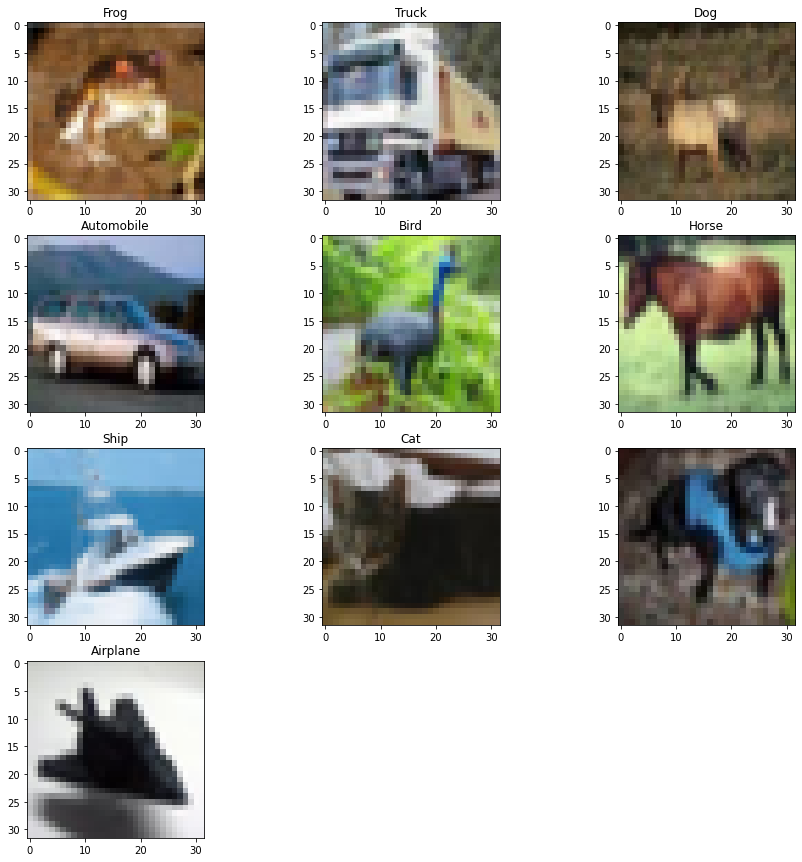
\includegraphics[width=0.9\textwidth]{CIFAR_images.png}
\end{figure}

\noindent
Even though half the data is not vehicle-related, a vehicle classification task would also be possible by removing all the animals data. Nevertheless, the whole data-set was still used for this research.

\subsection{MIO-TCD}
The data-set was used for the Traffic Surveillance Workshop and Challenge (TSWC) 2017, containing 648959 images of 11 classes, most of which are related to vehicles. Some sample images can be viewed in Figure \ref{img:MIOTCD-images}.

\begin{figure}[h]
\caption{Sample images from MIO-TCD data-set}
\label{img:MIOTCD-images}
\centering
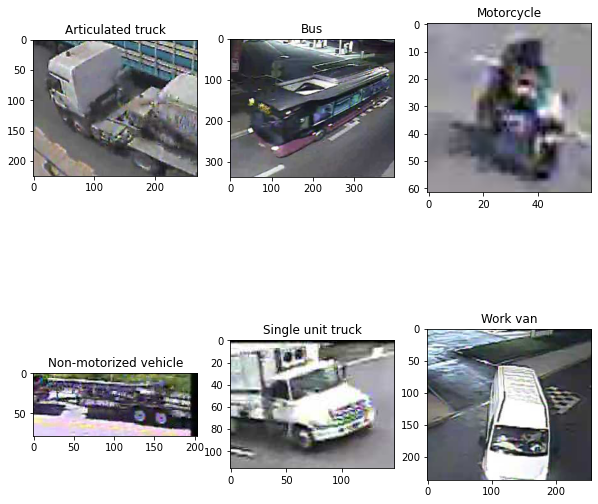
\includegraphics[width=0.75\textwidth]{MIOTCD_images.png}
\end{figure}

\noindent
Given the large size of the data-set, some classes have been removed for this test to lower the preprocessing and training time, particularly those that are not vehicles and one that contains too many samples. In the end, only the following classes were used: Articulated truck, Bus, Motorcycle, Non-motorized vehicle, Single unit truck, Work van.

\subsection{TAU-Vehicle}
This data-set comes from a contest during a Pattern Recognition course from Tampere Universities. It contains around 36000 images of 17 class: Ambulance, Boat, Cart, Limousine, Snowmobile, Truck, Barge, Bus, Caterpillar, Motorcycle, Tank, Van, Bicycle, Car, Helicopter, Segway, Taxi. Readers can refer to Figure \ref{img:TAU-images} for sample images.

\begin{figure}[h]
\caption{Sample images from TAU-Vehicle data-set}
\label{img:TAU-images}
\centering
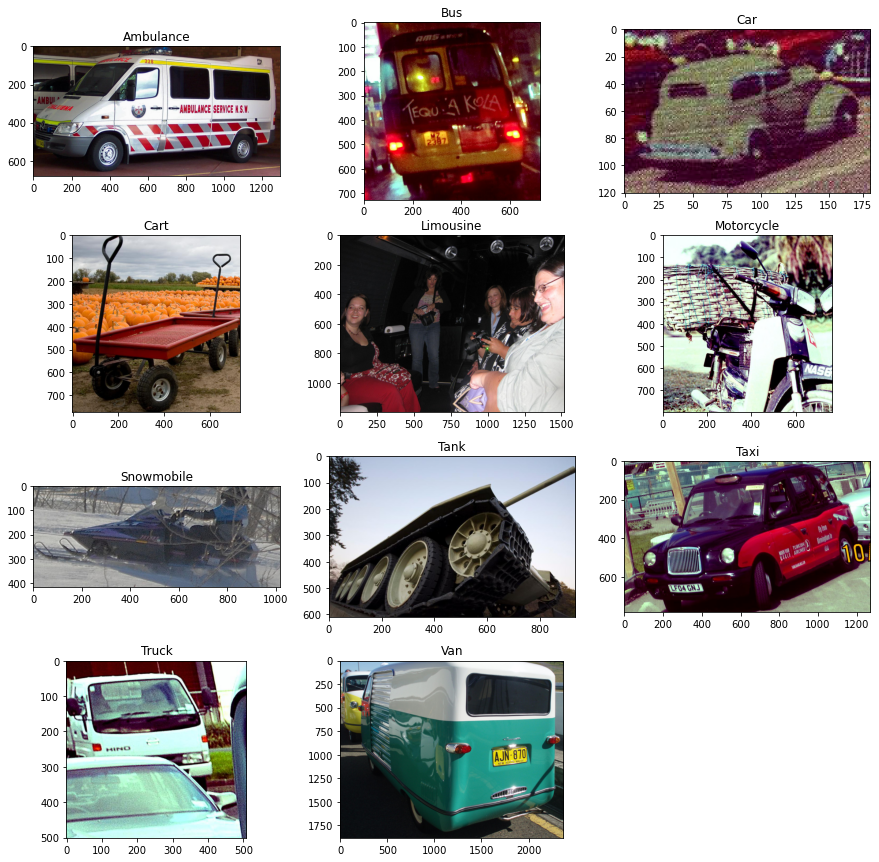
\includegraphics[width=0.9\textwidth]{TAU_images.png}
\end{figure}

\noindent
Similar to the MIO-TCD data-set, only the following classes were included: Ambulance, Bus, Car, Cart, Limousine, Motorcycle, Snowmobile, Tank, Taxi, Truck, Van.


\section{Algortihms}
This section introduces the algoriothms that have been used in the repository so far. Since the research focuses primarily on data lying on the Riemannian manifolds, only Riemannian-related algorithms will be discussed here.

\subsection{Multi-class Adaboost}
Adaboost is one algorithm from the Boosting \cite{Boosting} family, which combines a number of weak learners into one strong classifier. Though originally designed for binary classification, there have been attempts to make Adaboost work in the multi-class case, and one of them can be found in Algorithm 2 of \cite{Adaboost}. \\
However, for the algorithm to work with SPD matrices, small adjustments need to be made regarding the conversion of the inputs. This can be done by mapping the input data into a tangent plane on the manifold, which effectively returns the problem back to the usual vector case. To determine where the tangent plane should be, one can take the weighted mean of all the samples, and then project a tangent plane from that point, as can be seen from the algorithm below: \\

\begin{algorithm}[H]
    \KwIn{Training set ${(\bm{X_{i}}, y_{i})}_{i=1...N}$, $\bm{X_{i}} \in \mathcal{M}$, $y_{i} \in \{0, 1, ..., K\}$}
    \begin{enumerate}
    \item Initialize weights $w_{i} = 1/N$, $i = 1...N$\\
    \item Repeat for $m = 1, 2, ..., M$:
        \begin{enumerate}
        \item Compute weighted mean of the points $\bm{\mu_{m}} = \argmin_{\bm{X} \in \mathcal{M}} \sum_{i=1}^{N} w_{i}d^{2}(\bm{X_{i}}, \bm{X}) $\\
        \item Map data points to tangent space at $\bm{\mu_{m}}$\\
        \hspace{0.1cm} $\bm{x_{i}} = vec_{\bm{\mu_{m}}} (log_{\bm{\mu_{m}}}(\bm{X_{i}}))$\\
        \item Fit a classifier $T_{m}(x)$ to the training data using weights $w_{i}$\\
        \item Compute $err_{m} = \frac{\sum_{i=1}^{N} w_{i} \cdot 1_{\{y_{i} \neq T_{m}(\bm{x_{i}})\}}}{\sum_{i=1}^{N} w_{i}}$\\
        \item Compute $\alpha_{m} = \log(\frac{1 - err_{m}}{err_{m}}) + \log(K - 1)$\\
        \item Update weights $w_{i} = w_{i} \cdot \exp(\alpha_{m} \cdot 1_{\{y_{i} \neq T_{m}(\bm{x_{i}})\}})$ for $i = 1...N$\\
        \item Re-normalize weights $w_{i}$ \\
        \end{enumerate}
    \end{enumerate}
    \KwOut{$C(x) = \argmax_k \sum_{m=1}^{M} \alpha_{m} \cdot 1_{\{T_{m}(\bm{x}) = k)\}}$}
    \caption{Multi-class AdaBoost on Riemannian manifolds}
\end{algorithm}
\vspace{5mm}
\noindent
It is worth noting that the mean of the points change after each iteration due to the adjustment of the weights. The main idea of Adaboost is that after every boosting iteration (where a new classifier is trained), the weights of misclassified samples get bigger until they are correctly classified, thus making the later classifiers stronger after each iteration. Finally, the output of Adaboost is determined by a majority vote across all classifiers.


\subsection{Multi-class Logitboost}
Coming from the same family as Adaboost, Logitboost also leverages the idea of utilizing multiple weak learners, but instead it aims to minimize the negative binomial log-likelihood of the samples (see $p_{k}(x)$ below). \\

\begin{algorithm}[H]
    \KwIn{Training set ${(\bm{X_{i}}, y_{i})}_{i=1...N}$, $\bm{X_{i}} \in \mathcal{M}$, $y_{i} \in \{1, 2,..., K\}$}
    \begin{enumerate}
    \item Initialize weights $w_{ik} = 1/N$, probabilities $p_{k}(x) = 1/K$ and $F_{k}(x) = 0, i = 1...N, k = 1...K$\\
    \item Convert labels $y_{i}$ into one-hot encoded vectors:
        \begin{center}
            $y_{ik} = $
            $\begin{cases}
                1 \quad \text{ if } k = y_{i}, \\
                0 \quad \text{ otherwise}
            \end{cases}$
        \end{center}
    \item Repeat for $m = 1, 2, ..., M$:
        \begin{enumerate}
            \item Repeat for $k = 1, 2, ..., K$:
                \begin{enumerate}
                    \item Compute working responses and weights in the k-th class: \\
                    \begin{center}
                        $\bm{z_{ik}} = \frac{y_{ik} - p_{k}(x_{i})}{p_{k}(x_{i})(1 - p_{k}(x_{i}))}$ \\
                        $\bm{w_{ik}} = p_{k}(x_{i})(1 - p_{k}(x_{i}))$ \\
                    \end{center}
                    \item Compute weighted mean of the points $\bm{\mu_{mk}} = \argmin_{\bm{X} \in \mathcal{M}} \sum_{i=1}^{N} \bm{w_{ik}}d^{2}(\bm{X_{i}}, \bm{X}) $\\
                    \item Map data points to tangent space at $\bm{\mu_{mk}}$\\
                    \hspace{0.1cm} $\bm{x_{i}} = vec_{\bm{\mu_{mk}}} (log_{\bm{\mu_{mk}}}(\bm{X_{i}}))$\\
                    \item Fit $f_{mk}(x)$ by weighted least-squares regression of $\bm{z_{ik}}$ to $\bm{x_{i}}$ with weights $\bm{w_{ik}}$\\
                \end{enumerate}
            \item Set $f_{mk}(x) \leftarrow \frac{K - 1}{K} (f_{mk}(x) - \frac{1}{K} \sum_{k=1}^{K} f_{mk}(x))$ and $\bm{F}_{k}(x) \leftarrow \bm{F}_{k}(x) + f_{mk}(x)$
            \item Update $p_{k}(x) = \frac{e^{\bm{F}_{k}(x)}}{\sum_{k=1}^{K} e^{\bm{F}_{k}(x)}}$ (the softmax operation), $\sum_{k=1}^{K} \bm{F}_{k}(x) = 0$
        \end{enumerate}
    \end{enumerate}
    \KwOut{The classifier $\argmax_k \bm{F}_{k}(x)$}
    \caption{multi-class Logitboost on Riemannian manifolds}
\end{algorithm}
\vspace{5mm}
\noindent
One can see that compared to Adaboost, the Logitboost algorithm also contains the steps involving mapping the SPD matrices to vectors using tangent planes, although the order is slightly different. Although the accuracy of Logitboost is generally better than Adaboost, it suffers from computation issues, as the back-and-forth mapping of tangent planes happen for every class, in every iteration, making it very expensive as the number of samples and classes increase. With that in mind, kernel SVM was proposed as the next solution to circumvent this issue.


\subsection{Riemannian Gaussian Kernel SVM}
This method is not only less computationally expensive than the Boosting algorithms, but it also gives a more accurate representation of distances on the Riemannian manifold (geodesic distance). The kernel function and more specific information can be found in \cite{ped_detection}, and in the algorithm below: \\

\begin{algorithm}[H]
    \KwIn{Training set ${(\bm{X_{i}}, y_{i})}_{i=1...N}$, $\bm{X_{i}} \in \mathcal{M}$, $y_{i} \in \{1, 2,..., K\}$}
    \begin{enumerate}
        \item Determine $\gamma$, either manually or using the below formula (only for the Riemannian case):
            \begin{center}
                $\gamma = N [{\sum_{i=0}^{N} d^{2}_{L}(\bm{X_{i}, \Pi_{L}}(\{1/N, \bm{X_{i}}\}_{1 \leq i \leq N}))}]^{-1}$
            \end{center}
        \item Compute the Gaussian (or RBF) kernel function as:
            \begin{center}
                $k_{G}(\bm{X, Y}) = \exp(-\gamma d_{L}(\bm{X, Y}))$
            \end{center}
        \item Fit an SVM classifier using $k_{G}(\bm{X, Y})$ as the Gram matrix and labels $y_{i}$
    \end{enumerate}
    \KwOut{Prediction of the SVM classifier on the testing set}
    \caption{Multi-class kernel SVM on Riemannian manifolds}
\end{algorithm}
\vspace{5mm}
\noindent
The distance function $d_{L}$ mentioned above depends on where the data lies, it can be the typical l-norm for the Euclidean case, or it can be the geodesic distance in the Riemannian world:
\begin{center}
    $d_{L}(\bm{X, Y}) = \|\log(\bm{X}^{1/2}\bm{YX}^{1/2})\|_{F}$
\end{center}
The value of $\gamma$ determines the extent to which a sample affects the others. According to \cite{sklearn_api}, higher $\gamma$ values lead to samples having to be closer to affect each other.

\section{Methodologies}
Since a test set was only available for some of the data-sets (mostly due to the them being in a contest, so the test labels are not given), different methods of benchmarking were used to assert the accuracy of the algorithms. The details are given in Table \ref{tab:method-table}.

\begin{table}[hbt!]
\centering
\caption{Methods used for each data-set}
\label{tab:method-table}
\begin{tabular}{llll}
\hline
\textbf{data-set}    & \multicolumn{1}{c}{\textbf{\# Train}} & \multicolumn{1}{c}{\textbf{\# Test}} & \multicolumn{1}{c}{\textbf{\# Classes}} \\ \hline
CIFAR-10            & 60000                                 & 10000                                & 10                                      \\
MIO-TCD             & 41478                                 & 5-fold CV                            & 7                                       \\
TAU Vehicle         & $\sim$36000                           & 5-fold CV                            & 17                                      \\
\end{tabular}
\end{table}
\vspace{5mm}
\noindent
These data-sets were then converted into 8x8 covariance descriptors, which lie in the Riemannian manifold space. To test the methods in the normal Euclidean (vector) space, the top half of the matrices were flattened (including the diagonal) to a 36-wide vector due to the semi-positive-definiteness nature of the matrices.

After preprocessing the data-sets to produce the Euclidean and Riemannian features, multi-class Logitboost and Adaboost algorithms were applied to both features with 2 different types of base estimator, 2-node and 8-node stumps, respectively. The accuracy is then obtained using the first 50, 100 and 200 iterations of each algorithm. 

Additonally, multi-class kernel SVM was used as the third algorithm in the experiment. The general idea of the SVM is that the samples will be converted into a Gram matrix containing the "distance" between one and the rest of the samples. In total, 2 Gram matrices will be made for each run, one comparing the training set with itself, while the other comparing the training with the test set. The only difference in the Riemannian and Euclidean is in how the "distance" is calculated, with the l2-norm and geodesic distance defined for the Euclidean and Riemannian case respectively.

\section{Results}
This section presents the results obtained from using the methods mentioned above, which can be found in Table \ref{tab:result-table}.

\begin{table}
\centering
\caption{Accuracy of classification algorithms}
\label{tab:result-table}
\begin{tabular}{lllllllll}
\hline
                                       & \textbf{}       & \multicolumn{1}{c}{\textbf{}}           & \multicolumn{3}{c}{\textbf{2 Terminal Nodes}}                                                         & \multicolumn{3}{c}{\textbf{8 Terminal Nodes}}                                                         \\
                                       & \textbf{Method} & \multicolumn{1}{c}{\textbf{Iterations}} & \multicolumn{1}{c}{\textbf{50}} & \multicolumn{1}{c}{\textbf{100}} & \multicolumn{1}{c}{\textbf{200}} & \multicolumn{1}{c}{\textbf{50}} & \multicolumn{1}{c}{\textbf{100}} & \multicolumn{1}{c}{\textbf{200}} \\ \hline
                                       & \multicolumn{2}{l}{\textit{\textbf{CIFAR-10}}}            &                                 &                                  &                                  &                                 &                                  &                                  \\
\multicolumn{1}{c}{\multirow{3}{*}{E}} & \multicolumn{2}{l}{Adaboost}                              & 0.252                           & 0.279                            & 0.302                            & 0.319                           & 0.342                            & 0.353                            \\
\multicolumn{1}{c}{}                   & \multicolumn{2}{l}{Logitboost}                            & 0.356                           & 0.377                            & 0.394                            & 0.405                           & 0.412                            & 0.397                            \\
\multicolumn{1}{c}{}                   & \multicolumn{2}{l}{RBF SVM}                               & \multicolumn{6}{c}{0.417}                                                                                                                                                                                     \\
\multirow{3}{*}{R}                     & \multicolumn{2}{l}{Adaboost}                              & 0.286                           & 0.319                            & 0.348                            & 0.355                           & 0.374                            & 0.392                            \\
                                       & \multicolumn{2}{l}{Logitboost}                            & 0.398                           & 0.420                            & 0.433                            & 0.443                           & 0.444                            & 0.435                            \\
                                       & \multicolumn{2}{l}{RBF SVM}                               & \multicolumn{6}{c}{0.457}                                                                                                                                                                                     \\
                                       &                 &                                         &                                 &                                  &                                  &                                 &                                  &                                  \\
                                       & \multicolumn{2}{l}{\textit{\textbf{MIO-TCD}}}             &                                 &                                  &                                  &                                 &                                  &                                  \\
\multirow{3}{*}{E}                     & \multicolumn{2}{l}{Adaboost}                              & 0.403                           & 0.417                            & 0.438                            & 0.515                           & 0.528                            & 0.523                            \\
                                       & \multicolumn{2}{l}{Logitboost}                            & 0.555                           & 0.579                            & 0.595                            & 0.682                           & 0.703                            & 0.717                            \\
                                       & \multicolumn{2}{l}{RBF SVM}                               & \multicolumn{6}{c}{0.372}                                                                                                                                                                                     \\
\multirow{3}{*}{R}                     & \multicolumn{2}{l}{Adaboost}                              & 0.434                           & 0.445                            & 0.467                            & 0.530                           & 0.543                            & 0.548                            \\
                                       & \multicolumn{2}{l}{Logitboost}                            & 0.586                           & 0.611                            & 0.630                            & 0.720                           & 0.741                            & 0.754                            \\
                                       & \multicolumn{2}{l}{RBF SVM}                               & \multicolumn{6}{c}{0.625}                                                                                                                                                                                     \\
                                       &                 &                                         &                                 &                                  &                                  &                                 &                                  &                                  \\
                                       & \multicolumn{2}{l}{\textit{\textbf{TAU-Vehicle}}}         &                                 &                                  &                                  &                                 &                                  &                                  \\
\multirow{3}{*}{E}                     & \multicolumn{2}{l}{Adaboost}                              & 0.413                           & 0.440                            & 0.414                            & 0.376                           & 0.358                            & 0.370                            \\
                                       & \multicolumn{2}{l}{Logitboost}                            & 0.533                           & 0.547                            & 0.555                            & 0.541                           & 0.530                            & 0.528                            \\
                                       & \multicolumn{2}{l}{RBF SVM}                               & \multicolumn{6}{c}{No data}                                                                                                                                                                                   \\
\multirow{3}{*}{R}                     & \multicolumn{2}{l}{Adaboost}                              & 0.452                           & 0.425                            & 0.405                            & 0.398                           & 0.397                            & 0.403                            \\
                                       & \multicolumn{2}{l}{Logitboost}                            & 0.566                           & 0.576                            & 0.584                            & 0.565                           & 0.558                            & 0.555                            \\
                                       & \multicolumn{2}{l}{RBF SVM}                               & \multicolumn{6}{c}{0.269}                                                                                                                                                                                     \\ \hline
\end{tabular}
\end{table}
\vspace{5mm}
\noindent
Overall, the Riemannian versions of the algorithms seem to perform better than their Euclidean counterpart, hinting that preserving the structure of the SPD matrices might play an important role in training the models. Additionally, increasing the number of iterations generally improves the accuracy of the predictions, but increasing the number of terminal nodes witness contradicting effects. While CIFAR-10 and MIO-TCD benefits ever so slightly from increasing the number of nodes, TAU-Vehicle does not seem to enjoy the increase in terminal nodes, and oftentimes in iterations as well.

\noindent
The accuracy score for the kernel SVM method is not very good at the moment, possibly due to the choice of gamma, or even the kernel itself. To improve the accuracy, one can try to sample multiple subwindows of an image, rather than using the whole image on its own. With this way, the number of available data will greatly increase, leading to more thorough training for the classifiers.

\noindent
No data can be retrieved for the kernel SVM case of the TAU-Vehicle data-set, due to the script timing out on the Triton machine. One possible solution is to try utilizing the GPU for rapid calculations, but it might take some time to get it running on Triton machines.

\newpage

\bibliographystyle{plain}
\bibliography{refs}

\end{sloppypar}
\end{document}
